
\section{Introduction to the PSoC microcontroller}

The first part of the lab is to help you familiarize yourself with the PSoC microcontroller. For students who have had the course ELEC-H-310, this will mainly be a reminder of the course's labs. 

You should start by installing the PSoC Creator IDE, as explained in Appendix~\ref{app:software_psoc}. If you are not confident with C programming, read \texttt{C\_language\_for\_uC.pdf}.

In the following subsections, you will learn how to instantiate and use some basic hardware components of the PSoC microcontroller: 
\begin{itemize}
	\item GPIOs (including LEDs and pushbuttons of the extension board); 
	\item the LCD screen; 
	\item the keyboard. 
\end{itemize}
You can always refer to refer to the PSoC tutorials (\url{www.cypress.com/psoc101}) or the datasheet of the hardware elements (these can be found by double-clicking on a component in the \texttt{TopDesign.cysch} file, and clicking on the button \texttt{Datasheet}). 




\subsection{General purpose input-output (GPIO)}

GPIOs are the most basic hardware elements, allowing to provide input commands to the microcontroller and receive output signals from the microcontroller. You can find tutorials of how to use GPIOs on the following website: 
\begin{itemize}
	\item \url{www.cypress.com/psoc101}, Lesson 1: ``1. Software Output Pins''
	\item \url{www.cypress.com/psoc101}, Lesson 2: ``2. Software Input Pins''
\end{itemize}
The following exercise will help you to interface two sort of IOs~: push-buttons and LEDs. The following (partial) list of functions are useful for using the GPIOs: 
\begin{itemize}
		\item \kw{gpioName\_Read()}: Read a GPIO value; 
		\item \kw{gpioName\_Write(value)}: Write a binary value to a GPIO;   
		\item \kw{CyDelay()}: use this function to put the microcontroller to sleep for a certain amount of milliseconds between two iterations of the for loop. 
\end{itemize}

\E{
\label{ex:1}
Open the \kw{Lab0} project. In this project, the different hardware components of the extension board have already been instantiated. 
\begin{itemize}
	\item Identify which hardware elements have been instantiated in the \texttt{TopDesign.cysch} file. You can have the details of a hardware component by double-clicking on it. 
	\item In the \texttt{Lab0.cydwr} file, the instantiated hardware elements have been associated with the pins of the PSoC microcontroller. Can you match the pin numbers of the PSoC with the hardware elements of the extension board by using the electrical schematics in Appendix~\ref{app:extension_psoc}? 
	\item Now write the code in the \texttt{main.c} file such that the LEDs D1-D4 turns on when the corresponding button SW1-SW4 is pushed, and turns off when this button is released. 
	\item Build, compile and load it on the PSoC board, then check its behavior (the shortcut buttons to build, compile and program the PSoC are located on the ribbon on the top left of the PSoC IDE). 
\end{itemize}
It is important to note that, in general, microcontroller are not designed to deliver high currents. If we were using high-brightness LEDs, we would need to use \textit{buffer} circuits (such as the \texttt{74ACT244}) to provide larger currents. 
}
{}






\subsection{LCD screen}

The LCD screen is a particular output that allows you to write characters on the 16-characters LCD screen, located on the extension board. By examining Appendix~\ref{app:extension_psoc}, you will notice that the LCD requires 7 output ports from the microcontroller. On the left side of the LCD screen, there is a potentiometer that allows you to control the contrast of the LCD screen. The 8 first characters of the LCD screen are defined to be row~0, the 8 last characters of the LCD screen are defined to be row~1. The exact mapping of the rows and columns of the LCD screen are shown in Figure~\ref{fig:lcd_screen}. 
\begin{figure}[h]
	\centering
	\includegraphics[width=4in]{lcd_screen.png}
	\caption{Row and column mapping of the LCD screen. }
	\label{fig:lcd_screen}
\end{figure}
The following (partial) list of functions are useful for using the LCD screen: 
\begin{itemize}
		\item \kw{LCD\_Init()}: to initialize the LCD; 
		\item \kw{LCD\_ClearDisplay()}: to clear the LCD display; 
		\item \kw{LCD\_Position()}: to control the cursor position of the LCD display; 
		\item \kw{LCD\_PrintString()}: to print a string of characters; 
		\item \kw{LCD\_PrintNumber()}: to print the decimal value of a 16-bit value; 
		\item \kw{LCD\_PrintInt8()}: to print a two-ASCII-character hex representation of the 8-bit value; 
		\item \kw{LCD\_PrintInt16()}: to print a four-ASCII-character hex representation of the 16-bit value; 
		\item \kw{LCD\_PutChar()}: to print \texttt{char} value; 
\end{itemize}

\E{
\label{ex:2}
Open the \kw{Lab0} project, which has already instantiated the LCD screen. Write a code such that counts the number of times that SW2 is pressed, and prints this value on the LCD screen under the format ``SW2 count: 8'' (where 8 should be replaced with the number of times SW2 is pressed). 
{}







\subsection{Keyboard}

A small $4\times 3$ keyboard is provided, that can be connected directly to the bottom of the extension board\footnote{there are 8 pins to the bottom of the extension board to allow for $4\times 4$ keyboards. Please use the seven leftmost pins for a $4\times 3$ keyboard. }. 
\begin{figure}[h]
	\centering
	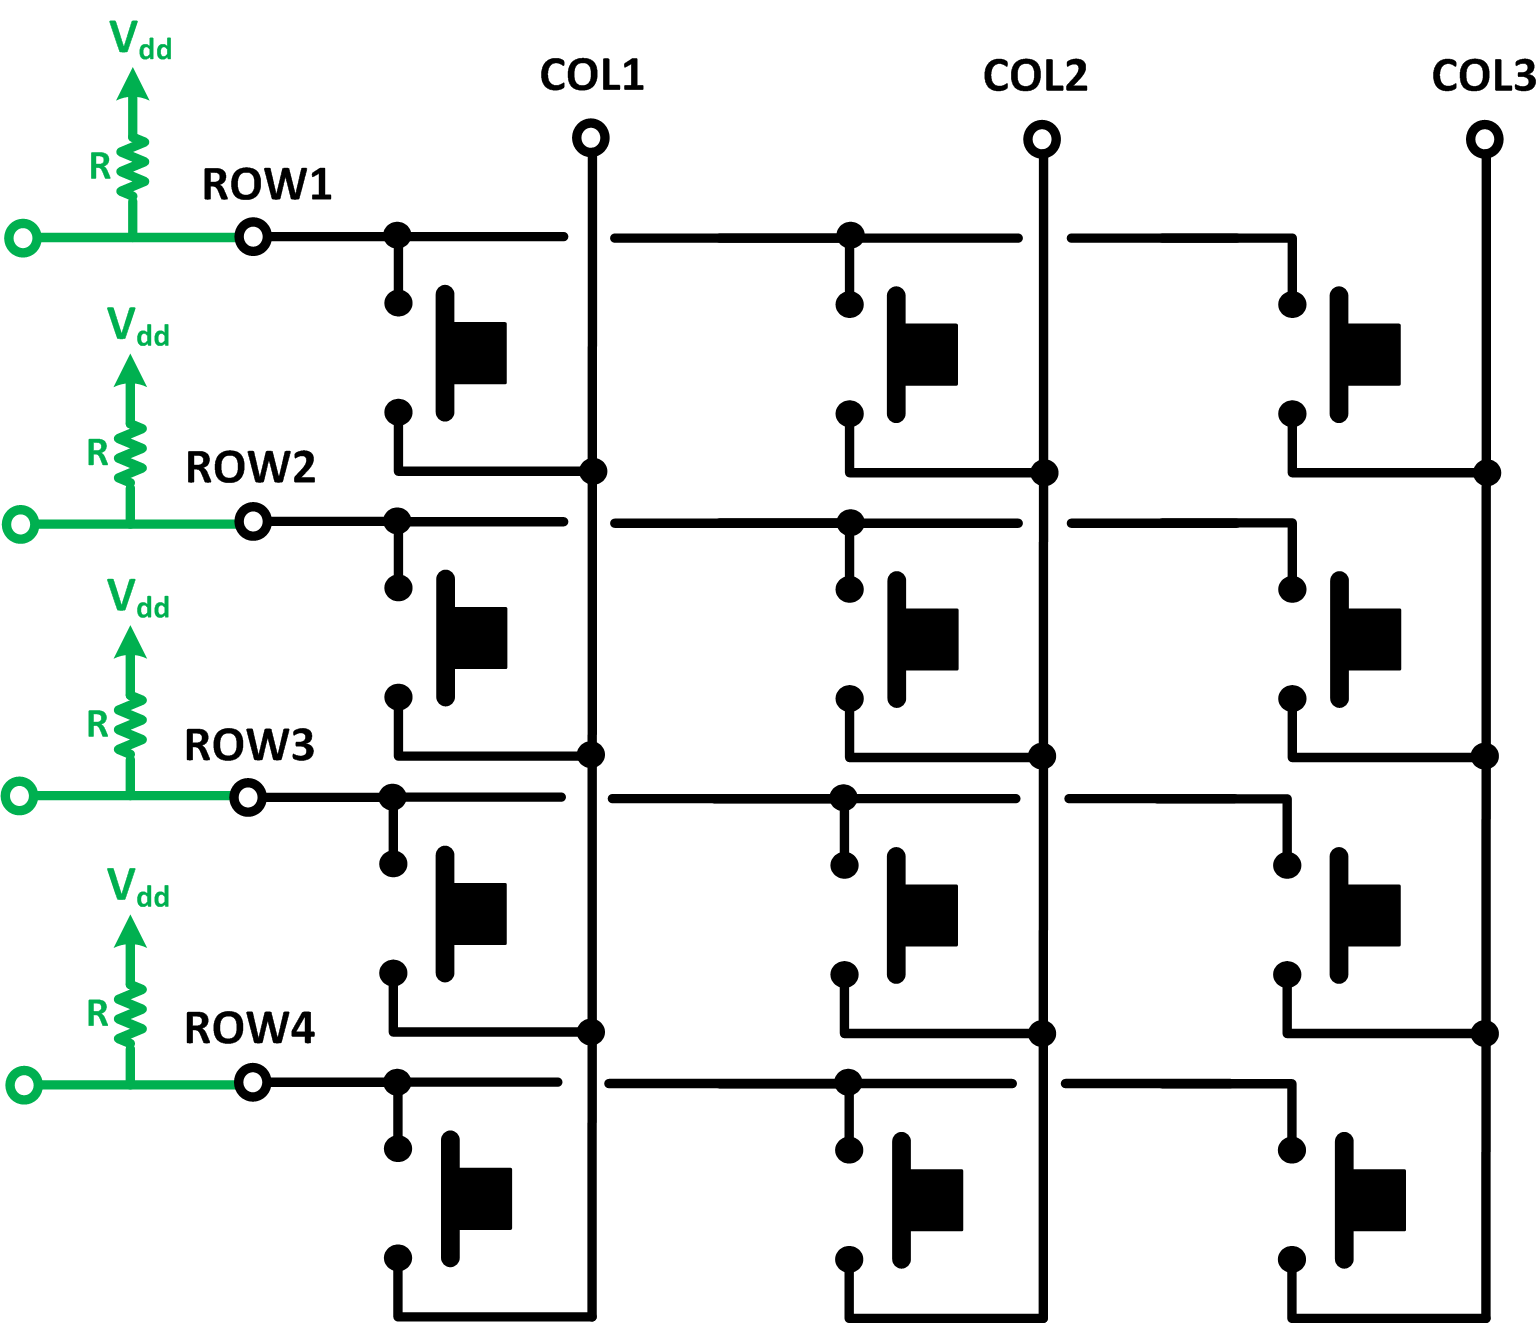
\includegraphics[width=2.5in]{keyboard.png}
	\caption{Electronic circuit of a $4\times 3$ keyboard. The green part represents the resistive pull-ups inputs of the PSoC board. }
	\label{fig:keyboard}
\end{figure}
A library has already been created and included in the project, and the keyboard has been instantiated in the \texttt{TopDesign.cysch} file. You can use the following function that are included in the library: 
\begin{itemize}
		\item \texttt{keyboard\_Start()} to initialize the keyboard; 
		\item \texttt{keyboard\_Scan()} to scan the keyboard. This will return the value that is pressed as a \texttt{uint8\_t}, and it will return the value \texttt{z} if no key is pressed. 
\end{itemize}

\E{
\label{ex:3}
Now write a code that prints successive pressed keys on the LCD screen. Your code should scan the keyboard every 50~ms. Note that if the keyboard is pressed only once, the value should be printed only once on the LCD screen. 
{}







